\subsection{Outline how the spin-orbit coupling arises. Discuss the resulting splitting of the energy states for the case of hydrogen.}


\paragraph{Spin-banekobling:}
Schrödingerligningen er en ikke-relativistisk ligning, så hvis man skal tilføje en relativistisk effekt, f.eks. spin, så skal dette manuelt gøres ved at tilføje dettes led i Hamiltonoperatoren. I stedet for at tilføje spin-banekoblingen og de relativistiske korrektioner hvert for sig, så findes disse på en og samme tid ved at gøre brug af den relativistiske ligning for det magnetiske felt, som funktion af det elektriske felt, \cref{eq:Q10_RelativistiskElektrodynamikMagnetiskOgElektriskFelt}.

For at motive brugen af en ligning for det magnetiske felt, så kigger vi på et atom, \cref{fig:Q10_SpinOrbitCouplingAtomFremDifferentPerspectives}(venstre), hvilket er illustreret, som vi kender det: En elektron i en cirkulær bane omkring en positiv kerne.
\begin{figure}[!h]
    \centering
    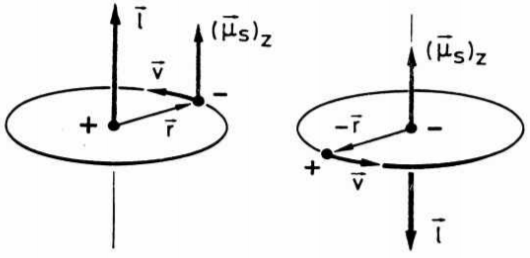
\includegraphics[width=0.7\textwidth]{Q10/images/SpinOrbiCouplingAtomFromDifferentPerspectives.PNG}
    \caption{Transformation fra kernens til elektronens perspektiv. Impulsmomentet tilhører, på begge figurer, partiklen, som er i banebevægelse, men er indtegnet ved dennes omdrejningspunkt. \textbf{Note:} Fjern fortegn fra $-\Vec{r}$ fra den højre figur, og dermed bliver $\Vec{l}$ også i retning opad i stedet.}
    \label{fig:Q10_SpinOrbitCouplingAtomFremDifferentPerspectives}
\end{figure}\\
Idet elektronen har et spin, så vil denne også have en $z$-kompenent af det magnetisk dipolmoment $\left(\Vec{\mu}_s\right)_z$. Siden elektronen er i cirkulær banebevægelse vil denne have et baneimpulsmoment $l$ (hvilket på \cref{fig:Q10_SpinOrbitCouplingAtomFremDifferentPerspectives}(venstre) er indtegnet ved elektronens omdrejningspunkt, altså atomets kerne), og dette baneimpulsmoment vil danne et magnetisk felt, som dipolmomentet så interagerer med.

Intuitivt giver det ikke mening, at elektronens dipolmoment skulle vekselvirke med elektronens dannede magnetiske felt, men dette vil give mening, når vi skifter perspektiv. Skifter vi nemlig perspektiv til at have elektronen i centrum, da vil kernen bevæge sig i cirkulær banebevægelse, hvilket vil give denne et impulsmoment, mens elektronen stadig har sit dipolmoment. Kernens impulsmoment vil nu skabe et magnetisk felt, hvilket elektronens dipolmoment vil interagere med.\\

Det giver altså mening, at vi vil kigge på den relativistiske ligning for magnetfeltet\footnote{An electron moving through an electric
field E experiences an effective magnetic field B given by this equation. This is a consequence of the way an electric field behaves under a Lorentz
transformation from a stationary to a moving frame in special relativity.}, da vi skal beskrive dipolmomentets interaktion med magnetfeltet:
\begin{align} \label{eq:Q10_RelativistiskElektrodynamikMagnetiskOgElektriskFelt}
    \Vec{B}_l &= -\frac{1}{c^2} \Vec{v} \cross \Vec{E} \: ,
\end{align}
hvor $\Vec{v}$ er elektronens hastighed.
Denne ligning kan omskrives ved at substituere $\Vec{E}$ med gradienten af potentialet og en enhedsvektor i den radielle retning (cylindriske koordinater):
\begin{align}
    \Vec{E} &= \frac{1}{e} \frac{\partial V}{\partial r} \frac{\Vec{r}}{r} \: ,
\end{align}
hvor $1/e$ kommer af, at elektrones potentielle energi $V$ er lig elektronens ladning ($-e$) gange det elektrostatiske potentiale. Derved bliver \cref{eq:Q10_RelativistiskElektrodynamikMagnetiskOgElektriskFelt}
\begin{align}
    \Vec{B}_l &= -\frac{1}{c^2} \Vec{v} \cross \left(\frac{1}{e} \frac{\partial V}{\partial r} \frac{\Vec{r}}{r}\right) = \frac{1}{c^2} \left(\frac{1}{e r} \frac{\partial V}{\partial r} \right) \Vec{r} \cross \Vec{v} = \frac{1}{m_e c^2} \left(\frac{1}{e r} \frac{\partial V}{\partial r} \right) \Vec{r} \cross m_e \Vec{v} \nonumber\\
    &= \frac{\hbar}{m_e c^2} \left(\frac{1}{e r} \frac{\partial V}{\partial r} \right) \Vec{l} \: ,
\end{align}
hvor det er blevet benyttet, at baneimpulsmomentet er $\hbar \Vec{l} = \Vec{r} \cross m_e \Vec{v}$.\\
Elektronens dipolmoment er givet ved
\begin{align} \label{eq:Q10_DipoleMomentOfAnElectron}
    \Vec{\mu}_s &= - g_s \mu_B \Vec{s} \: ,
\end{align}
hvor $g_s \simeq 2$ er Landé $g$-faktoren og $\mu_B = e\hbar/(2m_e)$ er Bohrmagnetonen.\\
Interaktionen mellem elektronens dipolmoment og det magnetiske felt giver da følgende Hamiltonoperator
\begin{align}
    H &= - \Vec{\mu}_s \cdot \Vec{B}_l = g_s \mu_B \Vec{s} \cdot \frac{\hbar}{m_e c^2} \left(\frac{1}{e r} \frac{\partial V}{\partial r} \right) \Vec{l}
\end{align}
hvilket er energien af kraftmomentet $\Vec{\mu}_s \cross \Vec{B}_l$, som den magnetiske dipol mærke i magnetfeltet $\Vec{B}_l$.

Vi har dog endnu ikke taget højde for, at vi har beregnet det magnetiske felt i et referencesystem, som ikke er statiornært, men som roterer, idet elektronen er i bevægelse omkring kernen. Dette hedder \emph{Thomas præcisionen}, og der kan tages højde for denne relativistiske effekt ved at erstatte $g_s$ med $g_s - 1$ (hvilket er $g_s - 1 \simeq 1$). Af dette fås Hamiltonoperatoren for spin-banekonlingen
\begin{align}
    H_{SO} &= (g_s - 1) \mu_B \Vec{s} \cdot \frac{\hbar}{m_e c^2} \left(\frac{1}{e r} \frac{\partial V}{\partial r} \right) \Vec{l} = (g_s - 1) \frac{e\hbar}{2m_e} \frac{\hbar}{m_e c^2} \left(\frac{1}{e r} \frac{\partial V}{\partial r} \right) \Vec{s} \cdot \Vec{l} \nonumber\\
    &= (g_s - 1) \frac{\hbar^2}{2m_e^2c^2} \left(\frac{1}{r} \frac{\partial V}{\partial r} \right) \Vec{s} \cdot \Vec{l} \: ,
\end{align}
hvor Bohrmagnetronen er indsat.\\


\paragraph{Spin-banekobling for hydrogen:}
For hydrogen er Coulombpotentialet
\begin{align}
    \frac{1}{r} \frac{\partial V}{\partial r} &= \frac{e^2}{4\pi\epsilon_0} \frac{1}{r^3} \: ,
\end{align}
så fra forventningsværdien af Hamiltonoperatoren får vi energiskiftet
\begin{align}
    E_{SO} &= \frac{\hbar^2}{2m_e^2c^2} \frac{e^2}{4\pi\epsilon_0} \braket{\frac{1}{r^3}} \braket{\Vec{s} \cdot \Vec{l} \:} \: ,
\end{align}
idet det er brugt, at $g_s - 1 \simeq 1$.

Integralet for $\braket{1/r^3}$ er givet ved
\begin{align}
    \braket{\frac{1}{r^3}} &= \dfrac{Z^3}{l\left(l+\dfrac{1}{2}\right)\left(l + 1\right) n^3a^3} \: ,
\end{align}
hvilket for hydrogen ($Z = 1$) er
\begin{align} \label{eq:Q10_<1/r^3>ForHydrogen}
    \braket{\frac{1}{r^3}} &= \dfrac{1}{l\left(l+\dfrac{1}{2}\right)\left(l + 1\right) n^3a^3} \: .
\end{align}

For at finde forventningsværdien $\braket{\Vec{s} \cdot \Vec{l} \: }$ skiftes basis til elektronens totale impulsmoment
\begin{align} \label{eq:Q10_TotalElektronimpulsmoment}
    \Vec{j} &= \Vec{l} + \Vec{s} \: ,
\end{align}
hvilket er en god basis, da Hamiltonoperatoren kommuterer med det totale elektronimpulsmoment, hvorfor $j$ er bevaret for et system uden påvirkning af eksterne kræfter. Spin-banekoblingen mellem $\Vec{l}$ og $\Vec{s}$ får disse to vektorer til at ændre deres retning samlet, således at deres sum er konstant lig $\Vec{j}$, hvorfor disse to vektoer præciserer rundt om $\Vec{j}$, som set på \cref{fig:Q10_TotalElektronimpulsmoment}.
\begin{figure}[!h]
    \centering
    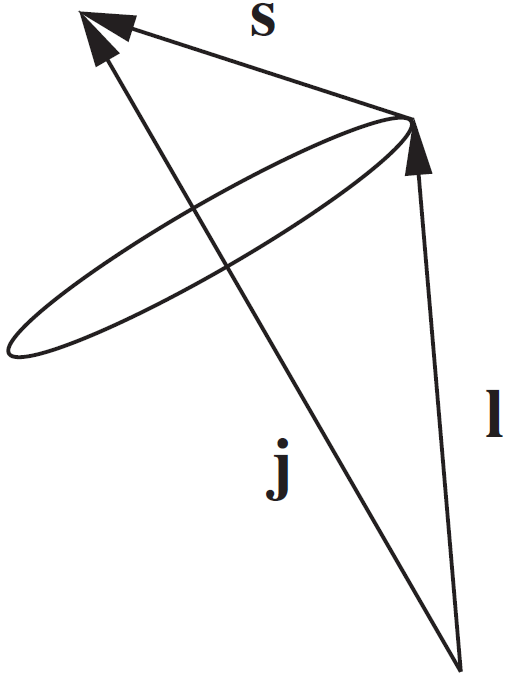
\includegraphics[width=0.23\textwidth]{Q10/images/AtomicQuantumNumberJ.PNG}
    \caption{Det totale elektronimpulsmoment $\Vec{j}$ findes som summes af baneimpulsmomentet $\Vec{l}$ og spinimpulsmomentet $\Vec{s}$, så $\Vec{j} = \Vec{l} + \Vec{s}$.}
    \label{fig:Q10_TotalElektronimpulsmoment}
\end{figure}\\
Kvadreres \cref{eq:Q10_TotalElektronimpulsmoment} fås
\begin{align}
    \Vec{j}^2 &= \Vec{l}^2 + \Vec{s}^2 + 2\Vec{s}\Vec{l} \nonumber\\
    \Rightarrow \Vec{s}\Vec{l} &= \dfrac{\Vec{j}^2 - \Vec{l}^2 - \Vec{s}^2}{2} \: ,
\end{align}
hvorfor forventningsværdien $\braket{\Vec{s} \cdot \Vec{l} \: }$ kan findes ud fra den kendte forventningsværdier $\braket{j^2}$, $\braket{l^2}$ og $\braket{s^2}$, så
\begin{align}
    \braket{\Vec{s} \cdot \Vec{l} \: } &= \frac{1}{2}\left\{j(j+1) - l(l+1) - s(s+1)\right\} \: .
\end{align}

Energiskiftet fra spin-banekoblingen bliver derved
\begin{align} \label{eq:Q10_EnergiskiftSpinOrbitForHydrogen}
    E_{SO} &= \frac{\beta}{2} \left\{j(j+1) - l(l+1) - s(s+1)\right\} \: ,
\end{align}
hvor
\begin{align}
    \beta &= \frac{\hbar^2}{2m_e^2c^2} \frac{e^2}{4\pi\epsilon_0} \dfrac{1}{l\left(l+\dfrac{1}{2}\right)\left(l + 1\right) n^3a^3} = \frac{\mu_B^2}{2c^2\pi\epsilon_0} \dfrac{1}{l\left(l+\dfrac{1}{2}\right)\left(l + 1\right) n^3a^3} \: .
\end{align}

\paragraph{Opsplitning af energitilstande i hydrogen:}